\section{HMM vs. MEMM}
\label{sec:comparison}

The HMM is generative model for the joint distribution of states (POS tags) and observations (words). The model is captured by two matrices, the transitional probability matrix for state to state and the emission probability matrix for state to observation. The state transition follows the Markov assumption. In other words, a the transitions between states is restricted to be dependent only on the immediate past~\cite{nlpBook}. On the other hand, MEMM is an extension of the maximum entropy classifier. It is a discriminative model that captures the conditional probability of the current state given the observation and the previous state. Figure \ref{hmmVmemm} shows pictorially the difference between the models. Both models can utilize a variation of Viterbi's algorithm to find the most likely sequence of tags for the observations (words) during decoding phase.

The MEMM, like the maximum entropy model it is based on, is a multinomial logistic regression for classification. It focuses on making the fewest number of assumptions about the training data. Furthermore, the HMM only uses two aspects of the problem: the transition probabilities for states $P( S_i | S_{i-1} )$ and the emission probabilities for the current state and observation $P( O_i | S_i )$. MEMM, in contrast, integrates feature information from the observations in addition to the previous state knowledge in order to derive a more accurate model. For example, capitalization is closely associated with proper nouns and specific suffixes, such as "-ed" and "-ing", tend to be associated with verbs. These rules are useful features that can help improve the accuracy of the POS tagger which are not captured in the HMM model. Moreover, this model can be augmented further to include features involving additional past states and past or future observations~\cite{nlpBook}. This behavior is captured in a single transitional probability matrix. Finally, the typical algorithms used to find the most probable state sequence for HMM can be modified for MEMM without additional overhead~\cite{memmPaper}.

However, MEMM is susceptible to the "label bias problem". This issue generally arises in two forms. First, if a state, $S_i$, has a high probability of transitioning to $S_j$ (low entropy with the extreme case of probability from $S_i$ to $S_j$ being 1), the observation would be less influential during the decoding task. In POS tagging this occurs when a sequence of observations and the corresponding tags appear frequently in the training set. The other source of bias is during labeling phase. When an observation occurs infrequently in the training set, it leads to an inaccurate prediction. Consequentially, the error propagates to subsequent observations \cite{labelBiasProblem}.

\begin{figure}[ht]
\centering
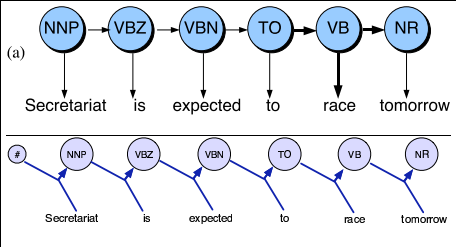
\includegraphics[width=80mm]{figures/memm.png}
\caption{(top) Hidden Markov Model and (bottom) Maximum Entropy Markov Model~\cite{nlpBook}. \label{hmmVmemm}}
\end{figure}
